% ROZDZIAŁ 3: Model matematyczny i projekt regulacji

\chapter{Model matematyczny i projekt regulacji}
\label{ch:model}

Rozdział ten przedstawia wyprowadzenie modelu matematycznego układu kulka na belce,
metodę identyfikacji jego parametrów oraz projekt regulatorów PID i~LQR.

% -----------------------------------------------------------------------
\section{Model matematyczny obiektu regulacji}
% -----------------------------------------------------------------------

Układ składa się z~trzech elementów połączonych szeregowo: serwomechanizmu,
mechanicznego połączenia dźwigniowego oraz kulki toczącej się po belce.

\subsection{Dynamika serwomechanizmu}

Dynamikę serwomechanizmu w~pierwszym przybliżeniu opisuje człon inercyjny
pierwszego rzędu:
\begin{equation}
  G_{\mathrm{serwo}}(s) = \frac{\Theta_{\mathrm{serwo}}(s)}{\Theta_{\mathrm{ref}}(S)} = \frac{1}{T_{\mathrm{serwo}}\,s+1},
\end{equation}
gdzie $T_{\mathrm{serwo}}$ jest stałą czasową serwa.

Na podstawie danych katalogowych serwomechanizmu MG946R
(0{,}20\,s/60° przy 4{,}8\,V; 0{,}11\,s/60° przy 6\,V)
interpolując dla napięcia 5\,V:
\begin{equation}
  V_{5\mathrm{V}} \approx 0{,}20 - \frac{0{,}09}{1{,}2} \cdot 0{,}2 \approx 0{,}185\,\mathrm{s}/60^{\circ}.
\end{equation}
Przyjęto stałą czasową $T_{\mathrm{serwo}} = 0{,}095\,\mathrm{s}$.

\subsection{Dynamika kulki na belce}

\subsubsection{Równanie ruchu — II zasada dynamiki}

\begin{figure}[H]
  \centering
  \includegraphics[width=0.5\linewidth]{3-model-matematyczny-i-projekt-regulacji/3-img/silybelka.png}
  \caption{Rozkład sił działających na kulkę na równi pochyłej}
  \label{fig:silybelka}
\end{figure}

Dla kulki toczącej się bez poślizgu po belce pochylonej pod kątem $\theta$
równanie ruchu postępowego wynosi:
\begin{equation}
  m\ddot{x} = m\,g\sin\theta - T,
\end{equation}
a równanie momentu obrotowego wokół osi kulki:
\begin{equation}
  T \cdot R = J\,\ddot{\alpha},
\end{equation}
gdzie $T$ — siła tarcia statycznego, $R$ — promień kulki, $J$ — moment bezwładności,
$\varepsilon = \ddot\alpha$ — przyspieszenie kątowe kulki.

\subsubsection{Warunek toczenia bez poślizgu}

Z~warunku $\ddot x = \ddot\alpha\cdot R$ eliminuje się siłę tarcia:
\begin{equation}
  m\ddot{x} + \frac{J}{R^2}\ddot{x} = m\,g\sin\theta
  \quad\Rightarrow\quad
  \ddot{x} = \frac{g\sin\theta}{1 + J/(mR^2)}.
\end{equation}

Dla małych kątów $\sin\theta\approx\theta$, a~dla kulki
$J = \tfrac{2}{3}mR^2$, stąd:
\begin{equation}
  \label{eq:ball_dyn}
  \ddot{x} = \underbrace{\frac{g}{1 + 2/3}}_{c_{\mathrm{ball}}} \cdot\theta
  = 0{,}6\,g\cdot\theta.
\end{equation}

Stała dynamiki kulki wynosi:
\begin{equation}
  c_{\mathrm{ball}} = 0{,}6 \times 9{,}81 = 5{,}886\,\mathrm{m/s^2}.
\end{equation}

\subsubsection{Transmitancja kulki na belce}

Po zastosowaniu względem \ref{eq:ball_dyn} transformaty Laplace'a (zerowe warunki początkowe) otrzymuje się:
\begin{equation}
  G_{\mathrm{ball}}(s) = \frac{X(s)}{\Theta_{\mathrm{beam}}(s)} = \frac{c_{\mathrm{ball}}}{s^2}.
\end{equation}

\subsection{Połączenie mechaniczne i transmitancja całkowita}

\begin{figure}[H]
  \centering
  \includegraphics[width=0.5\linewidth]{3-model-matematyczny-i-projekt-regulacji/3-img/kmech.png}
  \caption{Schemat mechanicznego połączenia serwa z~belką (dźwignia)}
  \label{fig:kmech}
\end{figure}

Kąty serwa i~belki powiązane są przez przekładnię mechaniczną:
\begin{equation}
  \theta_{\mathrm{beam}} = \frac{r_{\mathrm{serwo}}}{r_{\mathrm{belka}}} \cdot \theta_{\mathrm{serwo}}
  = k_{\mathrm{mech}} \cdot \theta_{\mathrm{serwo}},
\end{equation}
gdzie $r_{\mathrm{serwo}} = 3\,\mathrm{cm}$, $r_{\mathrm{belka}} = 15\,\mathrm{cm}$,
zatem $k_{\mathrm{mech}} = 0{,}2$.

Całkowita transmitancja układu (od sygnału sterującego $U(s)$ do pozycji kulki $X(s)$):
\begin{equation}
  G_{\mathrm{total}}(s) = k_{\mathrm{mech}} \cdot G_{\mathrm{serwo}}(s) \cdot G_{\mathrm{ball}}(s)
  = \frac{k_{\mathrm{mech}}\cdot c_{\mathrm{ball}}}{s^2(T_{\mathrm{serwo}}\,s+1)}.
  \label{eq:Gtotal}
\end{equation}

Podstawiając wartości liczbowe:
\begin{equation}
  G_{\mathrm{total}}(s) = \frac{0{,}2\cdot 5{,}886}{0{,}095\,s^3 + s^2}
  = \frac{1{,}177}{0{,}095\,s^3 + s^2}.
\end{equation}

% -----------------------------------------------------------------------
\section{Identyfikacja parametrów modelu}
% -----------------------------------------------------------------------

% ---------------------------------------------------------------
% SEKCJA 3.2 – Identyfikacja parametrów modelu
% Zastępuje dotychczasowe podrozdziały 3.2.1 (Sygnał PRBS) i 3.2.2
% Wkleić w miejsce \subsection{Sygnał PRBS} ... \subsection{Przyjęte parametry modelu}
% ---------------------------------------------------------------

% ---------------------------------------------------------------
% SEKCJA 3.2 – Identyfikacja parametrów modelu
% Zastępuje dotychczasowe podrozdziały 3.2.1 (Sygnał PRBS) i 3.2.2
% Wkleić w miejsce \subsection{Sygnał PRBS} ... \subsection{Przyjęte parametry modelu}
% ---------------------------------------------------------------

\subsection{Identyfikacja wzmocnienia metodą odpowiedzi skokowej}

\subsubsection{Metodyka pomiarowa}

W celu doświadczalnego wyznaczenia wzmocnienia statycznego układu przeprowadzono
eksperyment polegający na rejestracji odpowiedzi pozycji kulki na wymuszenia skokowe
kąta serwomechanizmu.
Punktem pracy (poziomem zerowym) przyjęto wysterowanie serwomechanizmu równe
$100\degree$, przy którym belka pozostaje w przybliżeniu pozioma.
Na wejście układu podawano kolejno skoki do pozycji $109\degree, 112\degree, 115\degree,
120\degree, 125\degree, 130\degree$ oraz $140\degree$.
Amplituda $A$ każdego wymuszenia stanowiła różnicę między zadaną pozycją a
poziomem zerowym (np.\ dla $125\degree$ wynosiła $A = 25\degree$).
W trakcie eksperymentu rejestrowano pozycję kulki na belce wyrażoną w milimetrach
w funkcji czasu.

\subsubsection{Analiza danych i estymacja wzmocnienia}

Dane pomiarowe zapisane w plikach CSV poddano obróbce w środowisku MATLAB.
W pierwszym kroku zwizualizowano surowe przebiegi i ręcznie wyznaczono okno
czasowe odpowiadające właściwemu ruchowi kulki -- od momentu inicjacji skoku do
chwili uderzenia kulki w ogranicznik belki.

Zgodnie z uproszczonym modelem  przyjęto, że
transmitancja łącząca kąt pochylenia belki z pozycją kulki ma postać podwójnego
całkowania:

\begin{equation}
    G(s) = \frac{K}{s^2}.
    \label{eq:Gident}
\end{equation}

W dziedzinie czasu odpowiada to równaniu różniczkowemu $\ddot{y}(t) = K \cdot u(t)$.
Przyłożenie na wejście funkcji skokowej o amplitudzie $A$ i dwukrotne scałkowanie
(przy zerowych warunkach początkowych) daje:

\begin{equation}
    y(t) = \frac{1}{2}\,K\,A\,t^2.
    \label{eq:yquad}
\end{equation}

Wycięty fragment danych scentrowano w punkcie $(0,\,0)$, a następnie za pomocą
funkcji \texttt{polyfit} wykonano aproksymację wielomianem drugiego stopnia
$y(t) = p_1 t^2 + p_2 t + p_3$.
Porównując współczynnik przy $t^2$ z równaniem~\eqref{eq:yquad} otrzymuje się:

\begin{equation}
    p_1 = \frac{1}{2}\,K\,A
    \qquad\Longrightarrow\qquad
    K = \frac{2\,p_1}{A}.
    \label{eq:Kest}
\end{equation}

Poniższy listing przedstawia fragment skryptu realizującego opisaną procedurę:

\begin{lstlisting}[language=Matlab, frame=single,
    caption={Fragment skryptu MATLAB estymującego wzmocnienie $K$},
    label={lst:matlab_ident}]
% Ograniczenie danych do wlasciwego ruchu pilki
idx = t_raw > 1.1 & t_raw < 2.2;
t = t_raw(idx);
y = y_raw(idx);

% Przesuniecie czasu i pozycji do zera
t = t - t(1);
y = y - y(1);

% Dopasowanie wielomianu 2. stopnia
p = polyfit(t, y, 2);

% Obliczenie wzmocnienia K
K_obl = (2 * p(1)) / A_stopnie;
\end{lstlisting}

\subsubsection{Weryfikacja wyników i wyznaczenie modelu końcowego}

Powyższą procedurę powtórzono dla wszystkich siedmiu wartości wychylenia.
Rysunki~\ref{fig:ident109}--\ref{fig:ident125} przedstawiają surowe przebiegi pozycji
kulki oraz dopasowane parabole dla kolejnych prób.

Zaobserwowano, że dla dużych kątów wychylenia estymowane wzmocnienie w największym
stopniu odbiega od wartości średniej.
Przyczyną jest niezerowa dynamika serwomechanizmu -- przy dużych skokach zadanej
pozycji kulka zaczyna się toczyć zanim serwo osiągnie wartość docelową, co narusza
założenie o skokowym charakterze wymuszenia i zaburza wyniki estymacji.
Z tego powodu z analizy wykluczono próby dla wychyleń $130\degree$ i $140\degree$,
pozostawiając pięć zestawów danych.

Wyznaczone wartości wzmocnienia dla pięciu uwzględnionych prób wynoszą:
\begin{equation}
    K_i = \bigl[11{,}9254;\;11{,}2886;\;12{,}2396;\;12{,}2772;\;11{,}9280\bigr].
    \label{eq:Klist}
\end{equation}

Końcową wartość wzmocnienia przyjęto jako średnią arytmetyczną powyższych próbek:
\begin{equation}
    K = 11{,}9318\;\frac{\mathrm{mm}}{\mathrm{s}^2\cdot\degree}.
    \label{eq:Kfinal}
\end{equation}

Transmitancja identyfikowanego układu kulka--belka przyjmuje zatem postać:
\begin{equation}
    G(s) = \frac{11{,}9318}{s^2}.
    \label{eq:Gfinal}
\end{equation}

Uzyskana wartość $K$ zastępuje teoretyczne $c_\mathrm{ball} \cdot k_\mathrm{mech}$
i stanowi podstawę do strojenia regulatorów PID i LQR opisanych w dalszej części
pracy.
Należy odnotować, że na dokładność estymacji wpływ ma ograniczona liczba prób
pomiarowych oraz ręczny dobór okna czasowego analizy -- dobór granic okna istotnie
oddziałuje na wyznaczoną wartość współczynnika $p_1$, a tym samym na końcowy wynik
uśredniania.

% --- Rysunki identyfikacyjne ---

\begin{figure}[H]
    \centering
    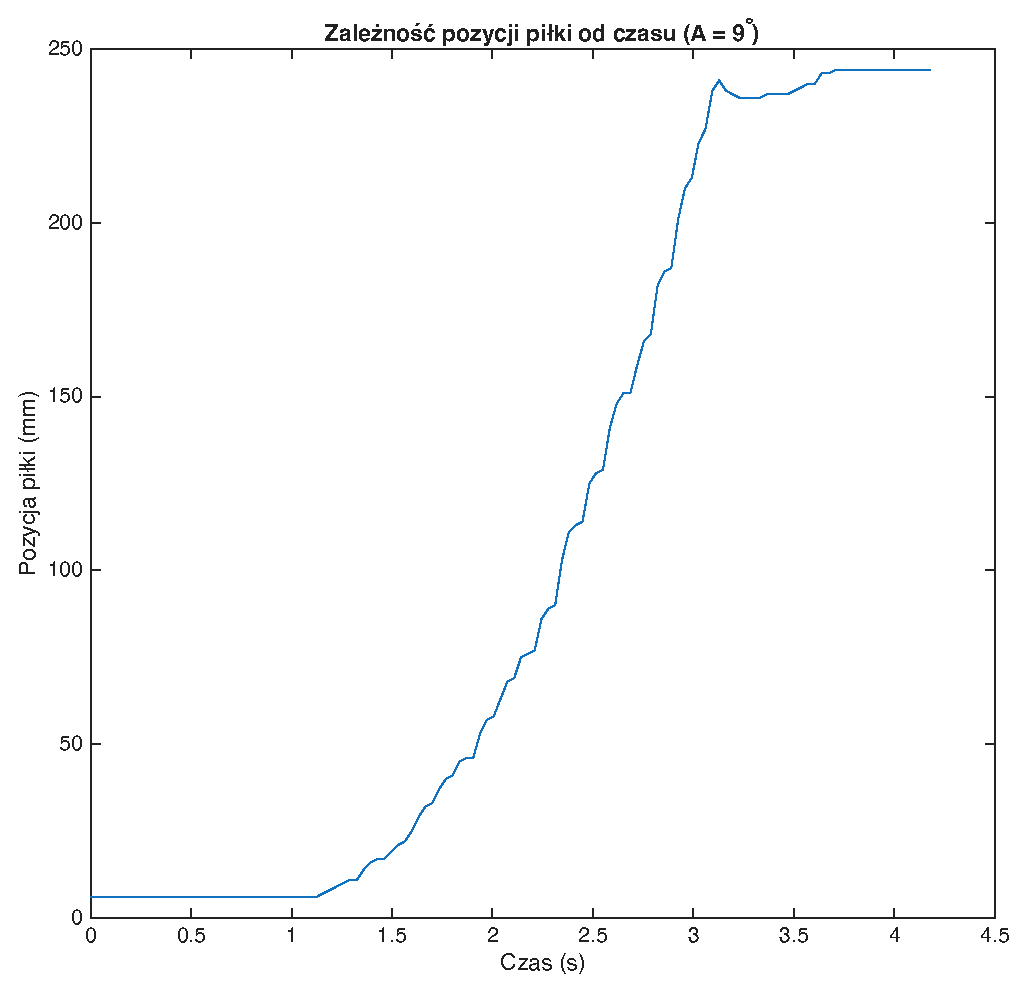
\includegraphics[width=0.6\textwidth]{3-model-matematyczny-i-projekt-regulacji/3-img/wykres_wychylenie_9.pdf}\\[4pt]
    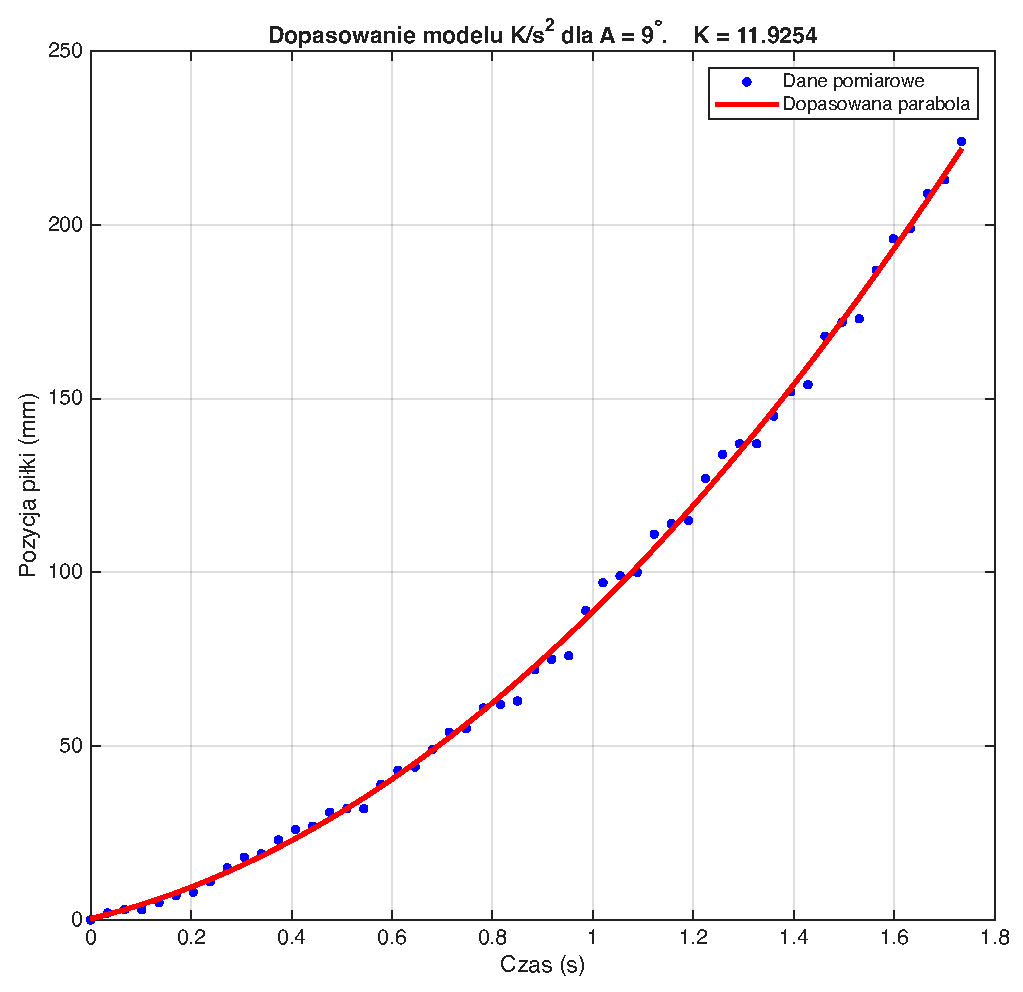
\includegraphics[width=0.6\textwidth]{3-model-matematyczny-i-projekt-regulacji/3-img/dopasowanie_109.pdf}
    \caption{Wyniki identyfikacji dla pozycji zadanej $109\degree$:
             surowe dane pozycji kulki (góra) oraz dopasowanie paraboliczne (dół).}
    \label{fig:ident109}
\end{figure}

\begin{figure}[H]
    \centering
    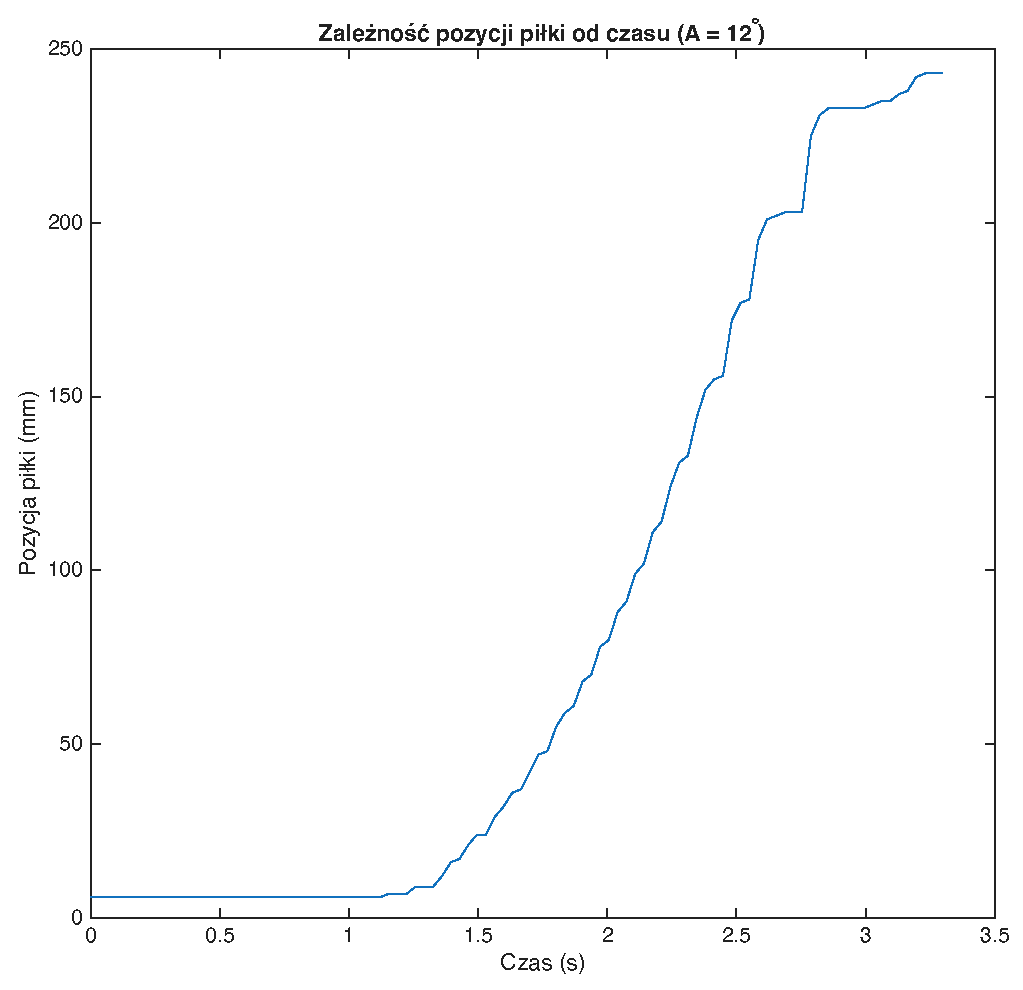
\includegraphics[width=0.6\textwidth]{3-model-matematyczny-i-projekt-regulacji/3-img/wykres_wychylenie_112.pdf}\\[4pt]
    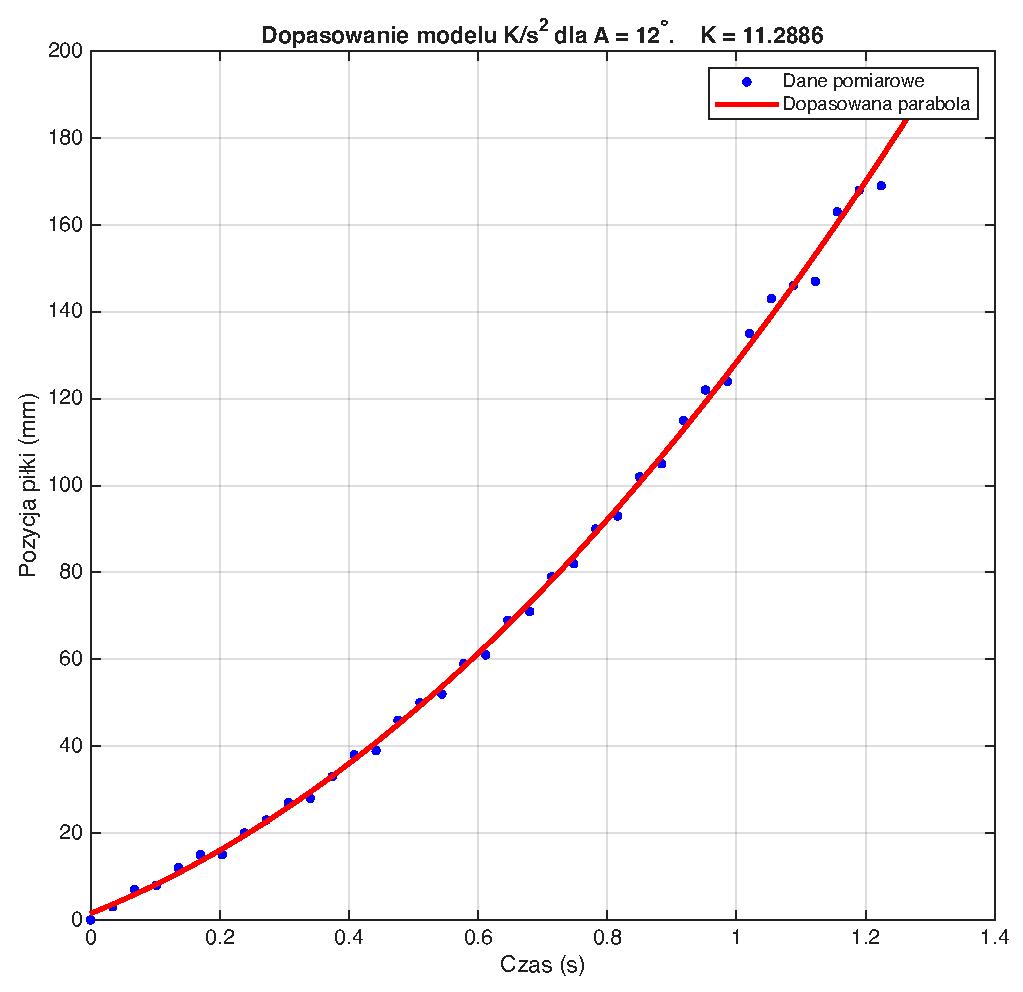
\includegraphics[width=0.6\textwidth]{3-model-matematyczny-i-projekt-regulacji/3-img/dopasowanie_112.pdf}
    \caption{Wyniki identyfikacji dla pozycji zadanej $112\degree$.}
    \label{fig:ident112}
\end{figure}

\begin{figure}[H]
    \centering
    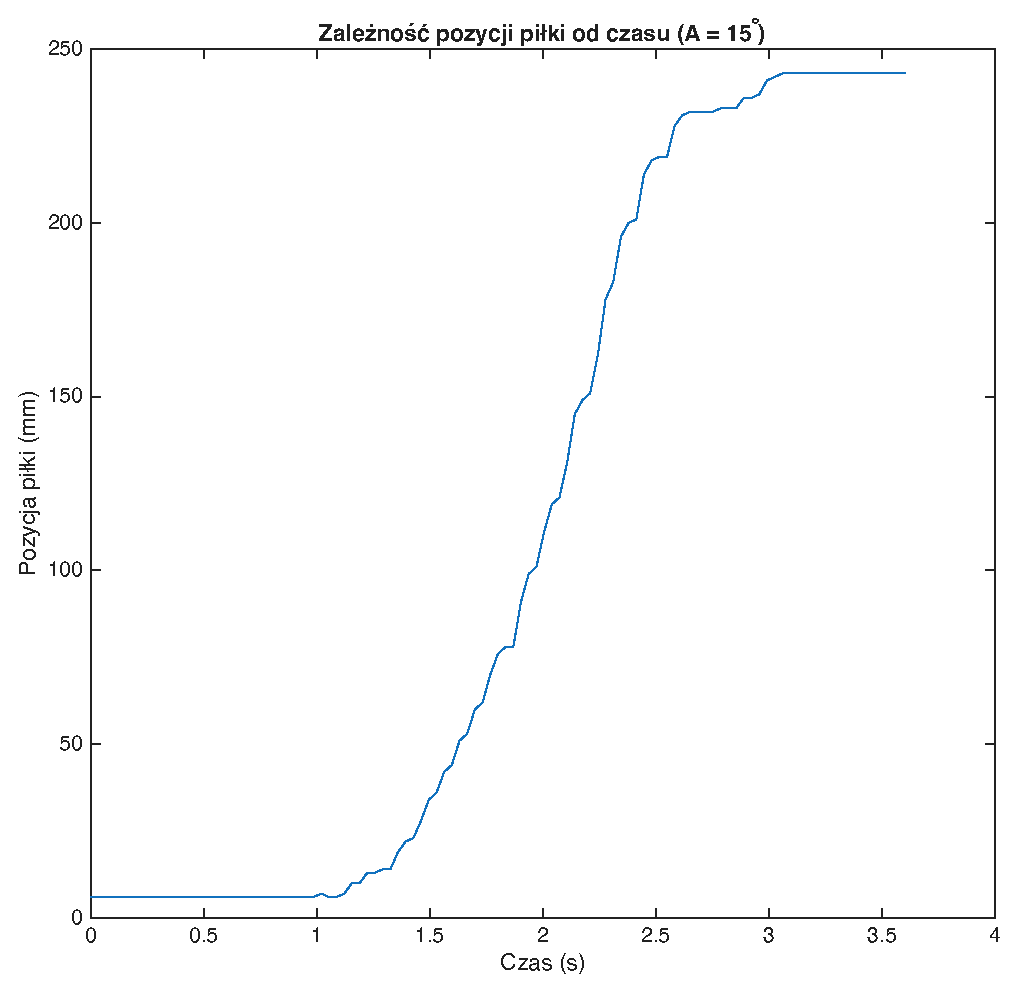
\includegraphics[width=0.6\textwidth]{3-model-matematyczny-i-projekt-regulacji/3-img/wykres_wychylenie_115.pdf}\\[4pt]
    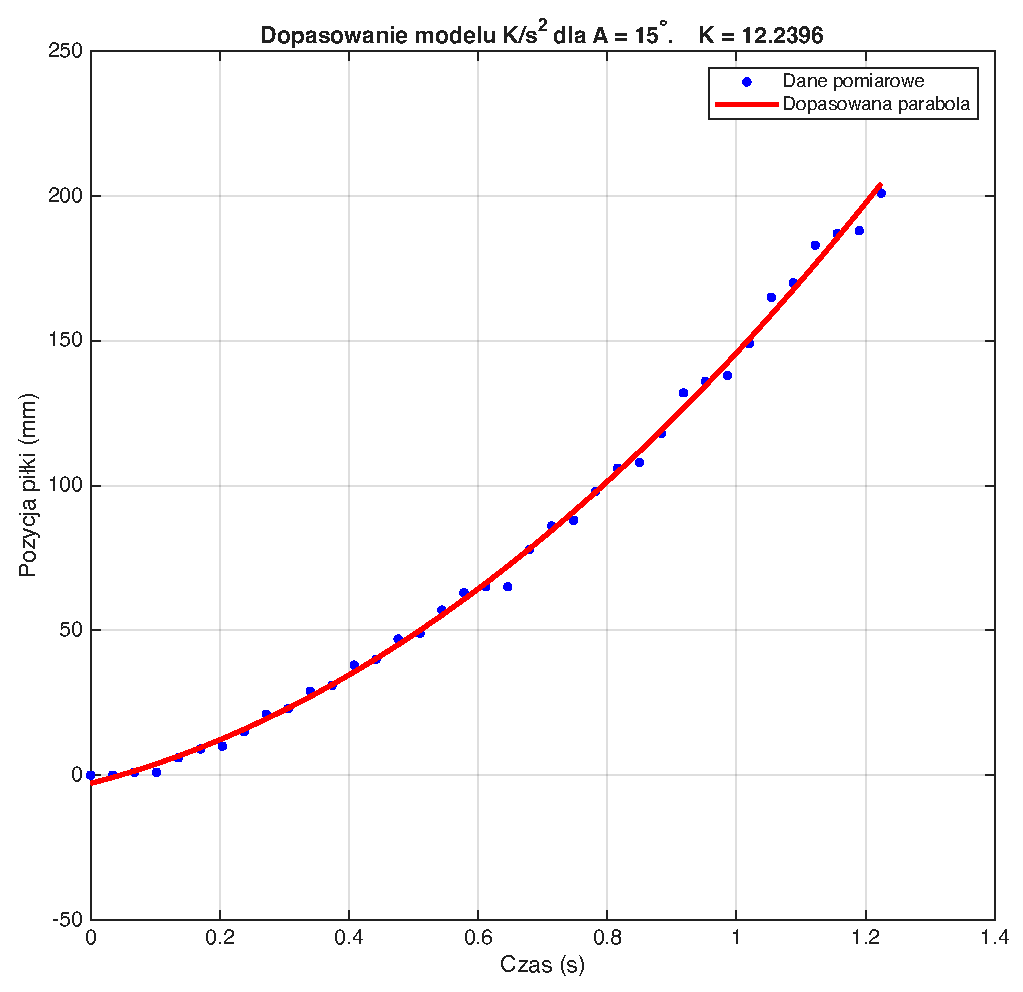
\includegraphics[width=0.6\textwidth]{3-model-matematyczny-i-projekt-regulacji/3-img/dopasowanie_115.pdf}
    \caption{Wyniki identyfikacji dla pozycji zadanej $115\degree$.}
    \label{fig:ident115}
\end{figure}

\begin{figure}[H]
    \centering
    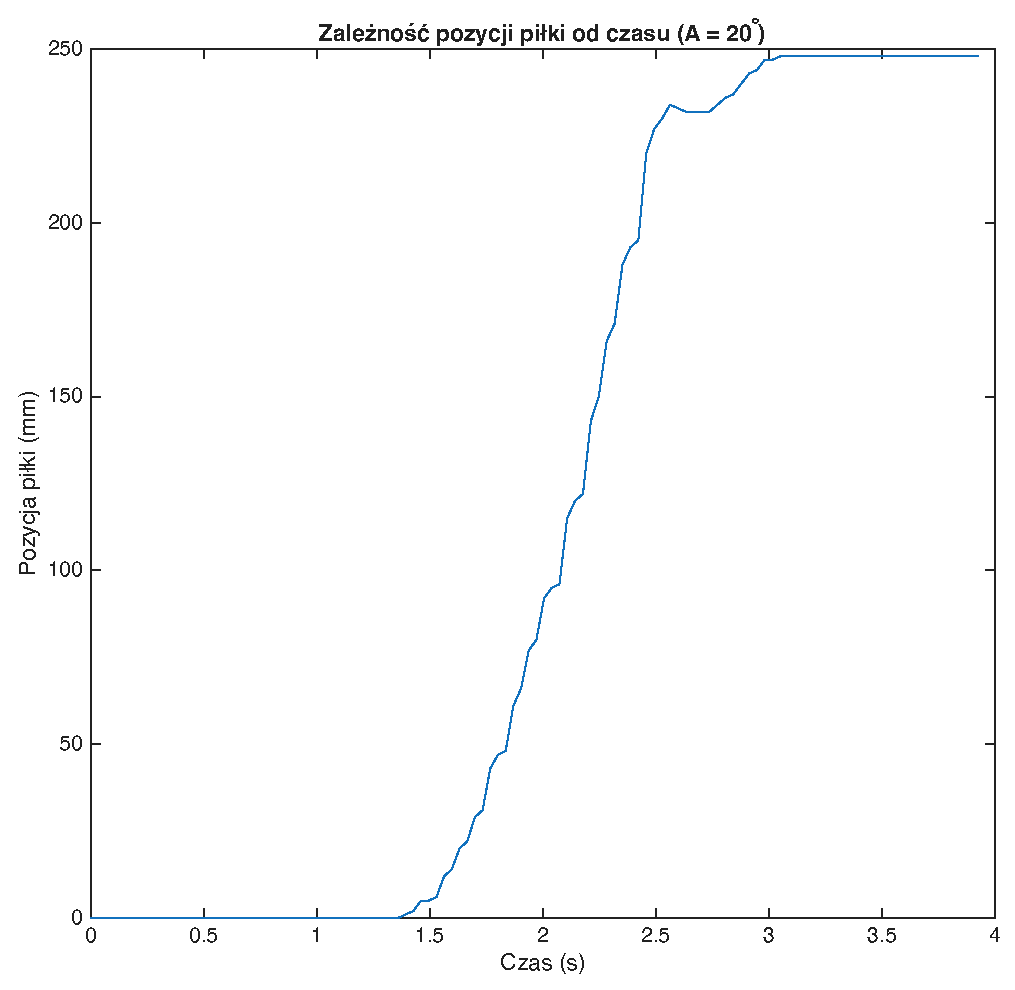
\includegraphics[width=0.6\textwidth]{3-model-matematyczny-i-projekt-regulacji/3-img/wykres_wychylenie_120.pdf}\\[4pt]
    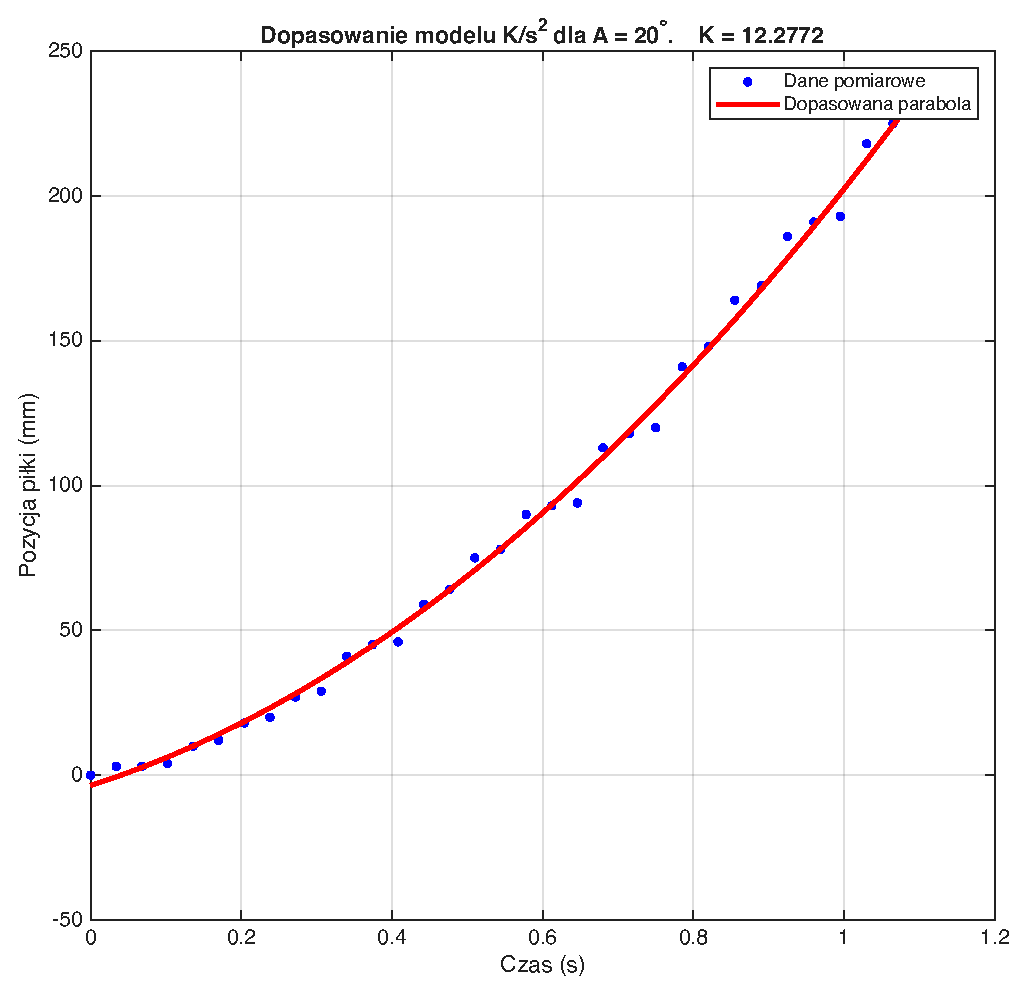
\includegraphics[width=0.6\textwidth]{3-model-matematyczny-i-projekt-regulacji/3-img/dopasowanie_120.pdf}
    \caption{Wyniki identyfikacji dla pozycji zadanej $120\degree$.}
    \label{fig:ident120}
\end{figure}

\begin{figure}[H]
    \centering
    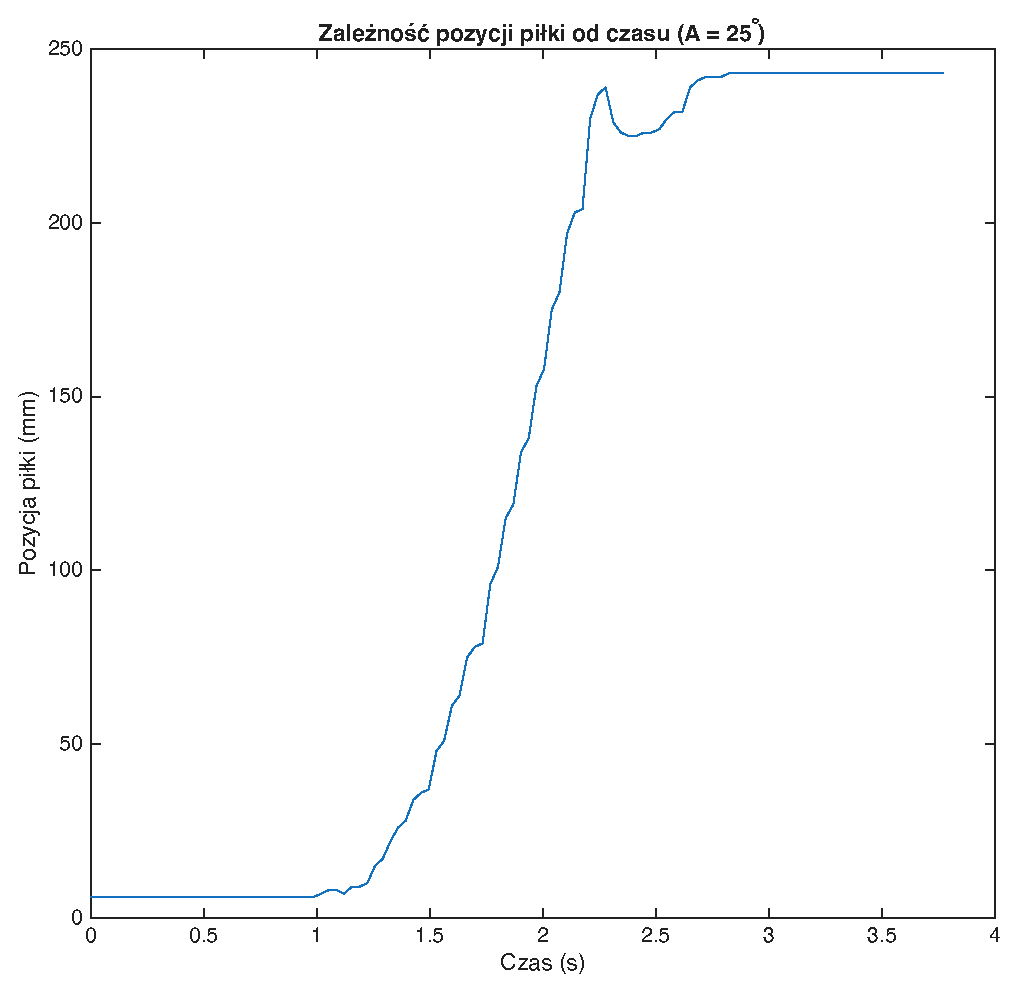
\includegraphics[width=0.6\textwidth]{3-model-matematyczny-i-projekt-regulacji/3-img/wykres_wychylenie_125.pdf}\\[4pt]
    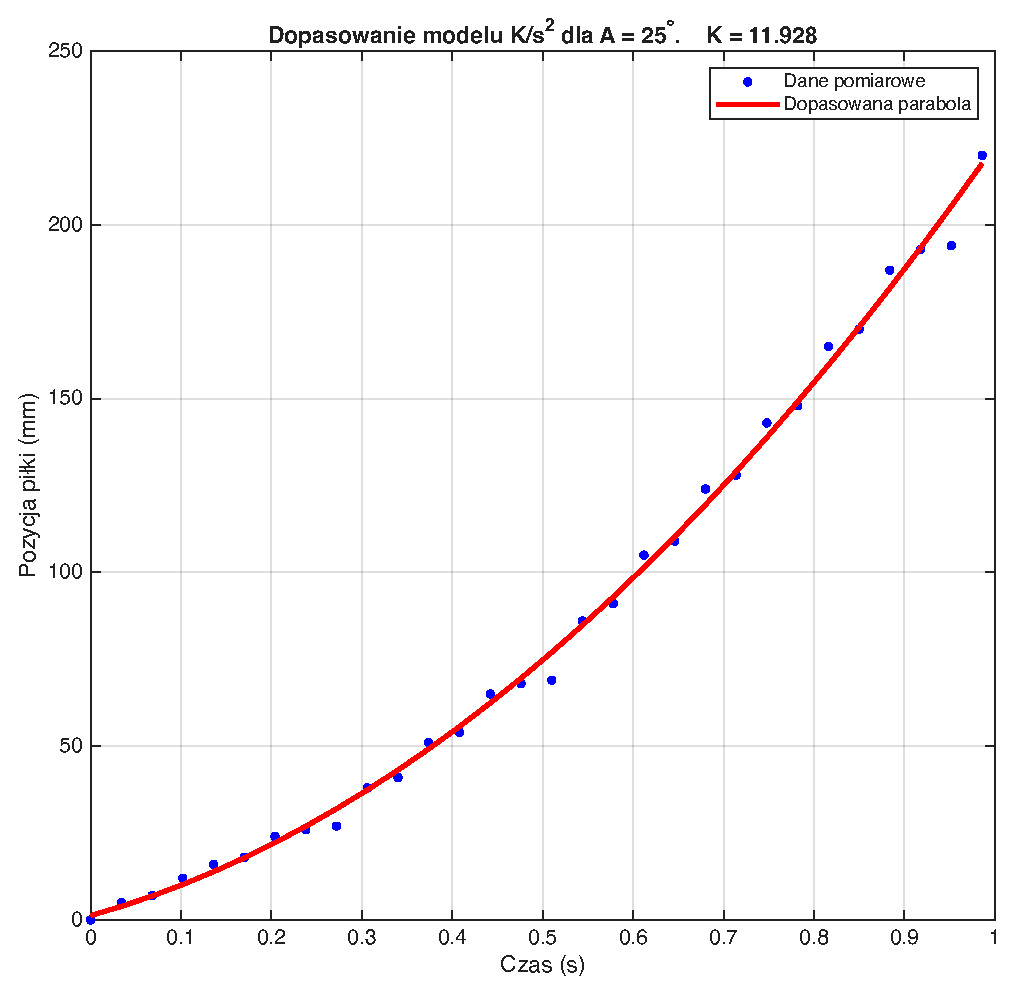
\includegraphics[width=0.6\textwidth]{3-model-matematyczny-i-projekt-regulacji/3-img/dopasowanie_125.pdf}
    \caption{Wyniki identyfikacji dla pozycji zadanej $125\degree$.}
    \label{fig:ident125}
\end{figure}

% Rysunki 130 i 140 stopni -- odrzucone z identyfikacji, ale zamieszczone
% dla kompletności (opcjonalnie - można usunąć bloki poniżej)
\begin{figure}[H]
    \centering
    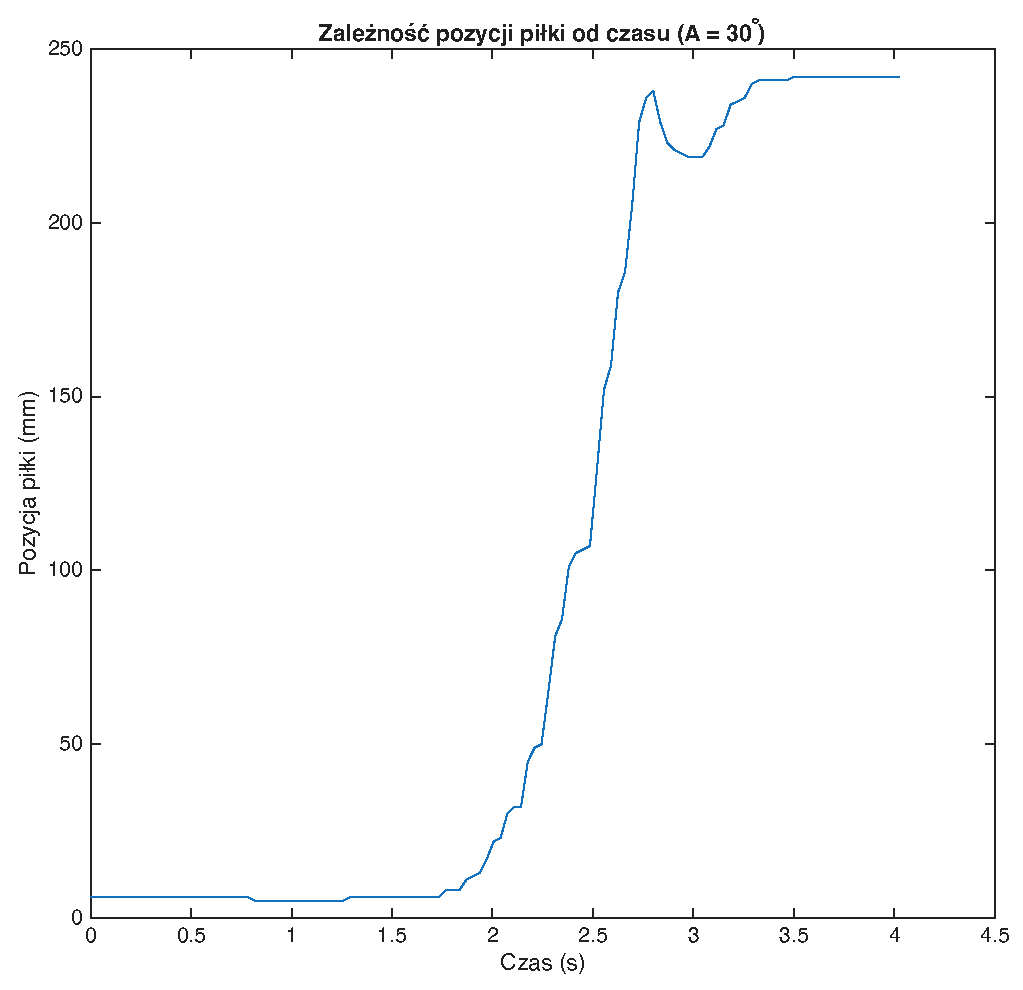
\includegraphics[width=0.6\textwidth]{3-model-matematyczny-i-projekt-regulacji/3-img/wykresy_wychylenie_130.pdf}\\[4pt]
    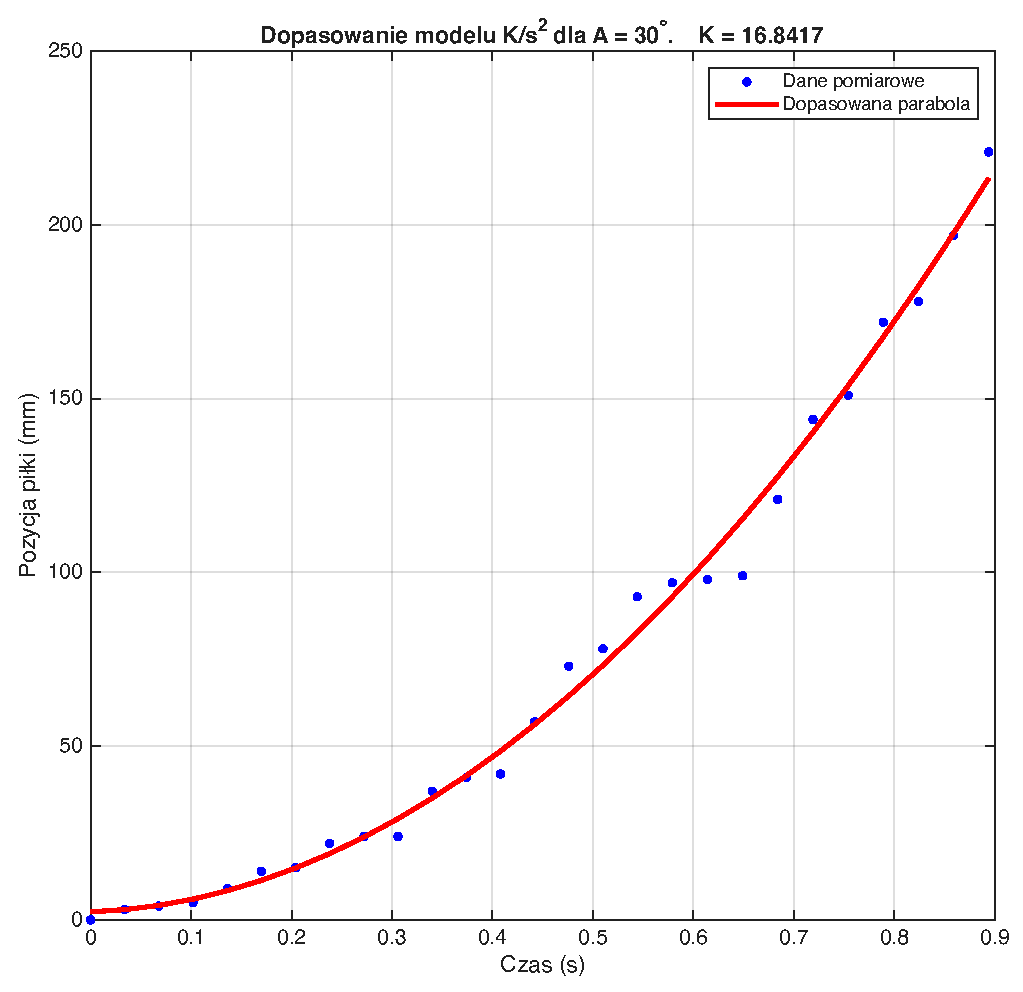
\includegraphics[width=0.6\textwidth]{3-model-matematyczny-i-projekt-regulacji/3-img/dopsaowanie_130.pdf}
    \caption{Wyniki dla pozycji zadanej $130\degree$ -- próba odrzucona
             z uwagi na widoczny wpływ dynamiki serwomechanizmu.}
    \label{fig:ident130}
\end{figure}

\begin{figure}[H]
    \centering
    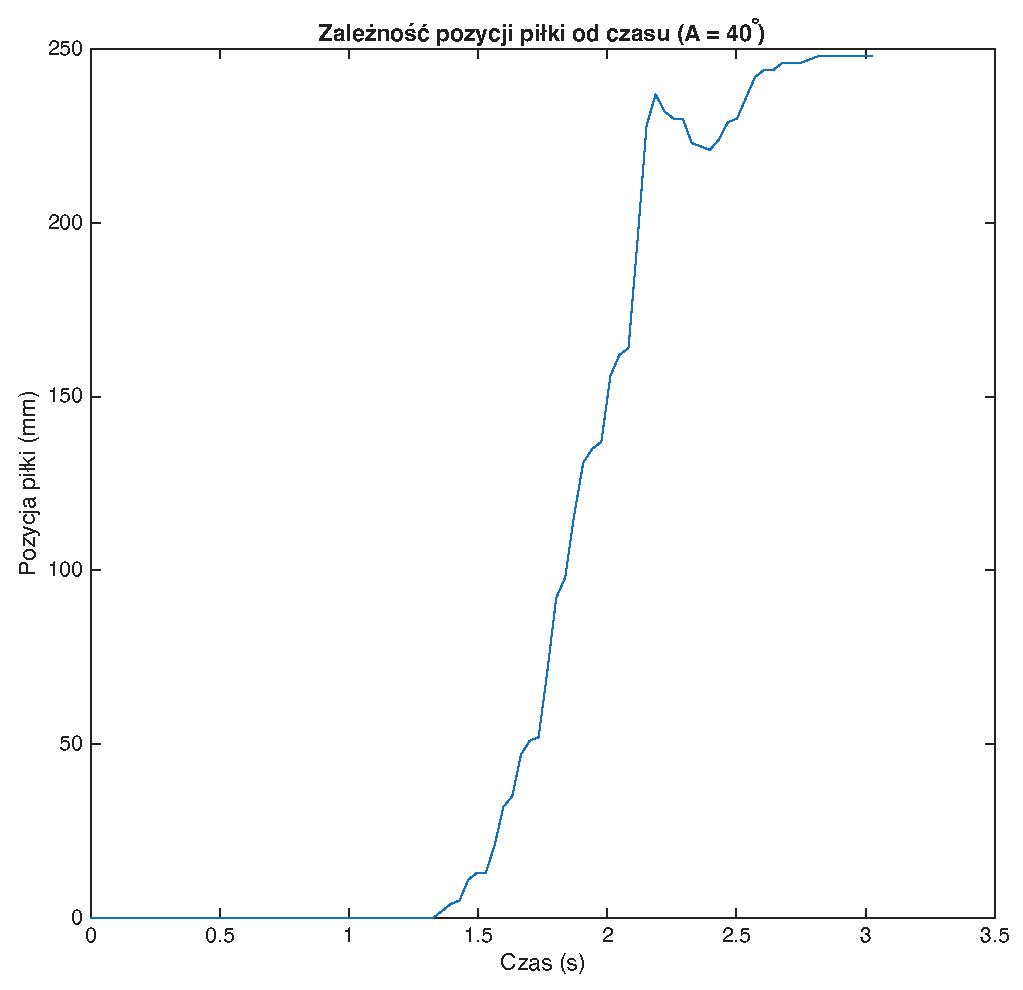
\includegraphics[width=0.6\textwidth]{3-model-matematyczny-i-projekt-regulacji/3-img/wychylenie_140_wykres.pdf}\\[4pt]
    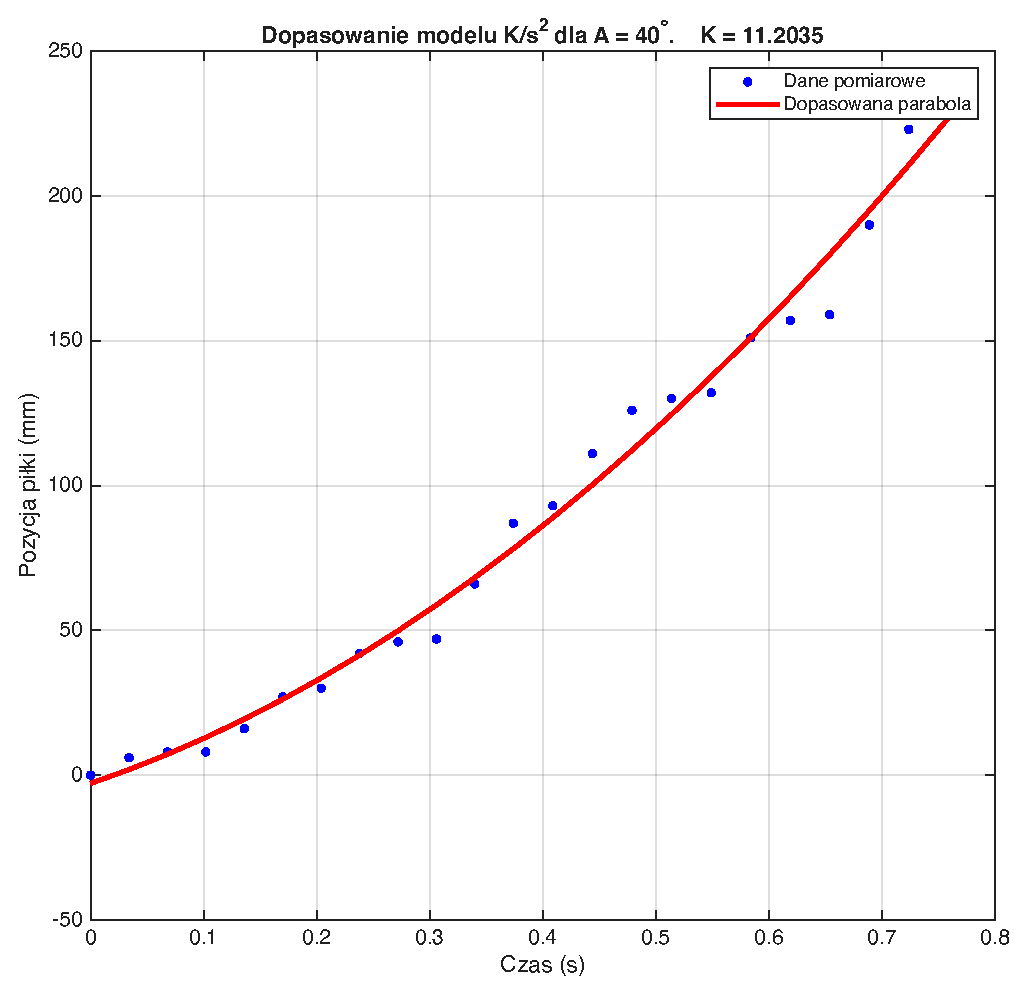
\includegraphics[width=0.6\textwidth]{3-model-matematyczny-i-projekt-regulacji/3-img/dopasowanie_140.pdf}
    \caption{Wyniki dla pozycji zadanej $140\degree$ -- próba odrzucona
             z uwagi na widoczny wpływ dynamiki serwomechanizmu.}
    \label{fig:ident140}
\end{figure}

% ---------------------------------------------------------------
% SEKCJA 3.2.2 – Przyjęte parametry modelu (aktualizacja tabeli)
% ---------------------------------------------------------------



\subsection{Przyjęte parametry modelu}

\begin{table}[H]
  \centering
  \caption{Parametry numeryczne modelu}
  \label{tab:parametry}
  \begin{tabular}{lll}
    \toprule
    \textbf{Parametr} & \textbf{Wartość} & \textbf{Źródło} \\
    \midrule
    $T_{\mathrm{serwo}}$ & $0{,}095\,\mathrm{s}$ & karta katalogowa, interpolacja \\
    $c_{\mathrm{ball}}$  & $5{,}886\,\mathrm{m/s^2}$ & wyprowadzenie analityczne \\
    $k_{\mathrm{mech}}$  & $0{,}20$ & pomiar geometryczny ($3\,\mathrm{cm}/15\,\mathrm{cm}$) \\
    \bottomrule
  \end{tabular}
\end{table}

TODO dokonczyc te sekcje!!!

% -----------------------------------------------------------------------
\section{Projekt regulatora LQR}
% -----------------------------------------------------------------------

\subsection{Opis przestrzeni stanów}

Jako wektor stanu przyjęto trzy fizycznie mierzalne wielkości:
\begin{equation}
  \mathbf{x} = \begin{bmatrix} x \\ \dot{x} \\ \theta \end{bmatrix},
\end{equation}
gdzie $x$ — pozycja kulki, $\dot{x}$ — prędkość kulki, $\theta$ — kąt belki.

Wyprowadzając równania różniczkowe z~bloków transmitancyjnych, otrzymuje się model
przestrzeni stanów w~postaci $\dot{\mathbf{x}} = A\mathbf{x} + Bu$, $y = C\mathbf{x}$:

\begin{equation}
  \begin{bmatrix} \dot{x}_1 \\ \dot{x}_2 \\ \dot{x}_3 \end{bmatrix}
  =
  \begin{bmatrix} 0 & 1 & 0 \\ 0 & 0 & c_{\mathrm{ball}} \\ 0 & 0 & -1/T_{\mathrm{serwo}} \end{bmatrix}
  \begin{bmatrix} x_1 \\ x_2 \\ x_3 \end{bmatrix}
  +
  \begin{bmatrix} 0 \\ 0 \\ k_{mech}/T_{\mathrm{serwo}} \end{bmatrix} u,
  \label{eq:statespace}
\end{equation}

\begin{equation}
  y = \begin{bmatrix} 1 & 0 & 0 \end{bmatrix} \mathbf{x}.
\end{equation}

Podstawiając wartości liczbowe ($c_{\mathrm{ball}} = 5{,}886$, $T_{\mathrm{serwo}} = 0{,}095$):

\begin{equation}
  A = \begin{bmatrix} 0 & 1 & 0 \\ 0 & 0 & 5{,}886 \\ 0 & 0 & -10{,}526 \end{bmatrix},
  \quad
  B = \begin{bmatrix} 0 \\ 0 \\ 10{,}526 \end{bmatrix},
  \quad
  C = \begin{bmatrix} 1 & 0 & 0 \end{bmatrix}.
\end{equation}

\subsection{Sterowalność}

Macierz sterowalności $\mathcal{C} = [B\;AB\;A^2B]$:

\begin{equation}
  \mathcal{C} = \begin{bmatrix}
    0       &  0       & 12{,}389 \\
    0       & 12{,}389 & -110{,}796 \\
    10{,}526 & -110{,}796 & 1{,}166\cdot10^3
  \end{bmatrix}.
\end{equation}

Wyznacznik:
\begin{equation}
  \det(\mathcal{C}) = 12{,}389 \times (-130{,}380) \approx -1614 \neq 0.
\end{equation}

Macierz ma pełny rząd~3, zatem układ jest \textbf{w~pełni sterowalny} —
możliwe jest zaprojektowanie efektywnego regulatora stanu (LQR).

\subsection{Obserwowalność}

Macierz obserwowalności $\mathcal{O} = \begin{bmatrix}
  C\\CA\\CA^2
\end{bmatrix}$

\begin{equation}
  \mathcal{O} = \begin{bmatrix}
    1 & 0 & 0 \\
    0 & 1 & 0 \\
    0 & 0 & 1{,}177
  \end{bmatrix}, \quad
  \det(\mathcal{O}) = 1{,}177 \neq 0.
\end{equation}

Rząd wynosi~3, układ jest \textbf{w~pełni obserwowalny} — wszystkie stany
można zrekonstruować z~pomiaru pozycji kulki $x$.

\subsection{Regulator LQR}

Regulator LQR (\textit{Linear Quadratic Regulator}) minimalizuje wskaźnik
jakości kwadratowej:
\begin{equation}
  J = \int_0^\infty \left( \mathbf{e}^T Q\,\mathbf{e} + u^T R\,u \right) dt,
\end{equation}
gdzie $\mathbf{e} = \mathbf{x} - \mathbf{x}_\mathrm{ref}$ jest wektorem uchybu stanu,
a~$\mathbf{x}_\mathrm{ref} = [r,\;0,\;0]^T$ odpowiada zadanej pozycji kulki~$r$,
zerowej prędkości i~zerowemu kątowi belki.

TODO dodac jakies przykladowe macierze Q i R / skrypt w pythonie gdzie to liczyliśmy 
musi to byc w tym miejscu

Uzyskany wektor wzmocnień $\mathbf{K}$ przeniesiono bezpośrednio do modułu
\texttt{lqr.c} firmware.
Sygnał sterujący wyznaczany jest jako:
\begin{equation}
  u = -\mathbf{K}\,\mathbf{e} = -[K_1\;K_2\;K_3]\begin{bmatrix} x - r \\ \dot{x} \\ \theta \end{bmatrix}.
\end{equation}


\section{Projekt regulatora PID}

W~firmware mikrokontrolera zaimplementowano klasyczny regulator PID
z~następującymi modyfikacjami:
\begin{itemize}
  \item \textbf{pochodna na pomiarze} — różniczkowanie sygnału wyjścia
        (nie uchybu), co eliminuje skok pochodnej przy zmianie wartości zadanej;
  \item \textbf{anti-windup} (ograniczenie członu całkującego) — zapobiega
        nasyceniu członu~I przy wysyceniu wyjścia;
  \item \textbf{dyskretyzacja} — metoda prostokątów (Euler przód)
        z~krokiem $T_s = 30\,\mathrm{ms}$.
\end{itemize}

TODO uzasadnic dlaczego pochodna na pomiarze i dokonczyć ten rozdzial task @Banaszak !!!!!!!

Nastawy regulatora PID ($K_p$, $K_i$, $K_d$) dobierane są iteracyjnie
i~przesyłane do mikrokontrolera w~czasie rzeczywistym przez aplikację
desktopową bez konieczności ponownego programowania układu.
